\section{Toric Code III, Berry Phase}

\subsection{Robustness of toric code GSD}
We saw the degeneracy of the toric code from both the explicit/formal calculation as well as from string operators. GSD in itself is not interesting, and is quite fragile; perturbations tend to split it - what is interesting about the TC GSD is that it is extremely robust; local perturbations cannot split it.

More precisely, consider an arbitrary local perturbation of $H$:
\begin{equation}
    H' = H + \lambda\sum_j V_j
\end{equation}
where $V_j$ is a local operator supported near site $j$.

\begin{center}
    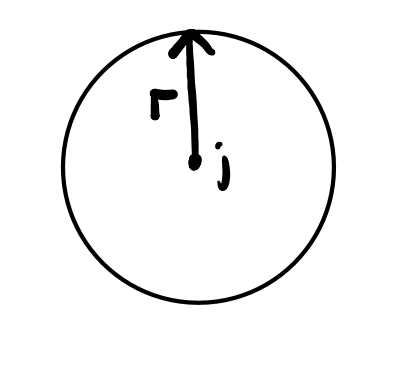
\includegraphics[scale=0.4]{Lectures/Images/lec3-local.png}
\end{center}

Claim: For sufficiently small $\lambda$, $H'$ has 4 nearly degenerate ground states with splitting:
\begin{equation}
    \delta \leq e^{-\text{C}(\lambda)L} 
\end{equation}
with $C(\lambda)$ a $\lambda$-dependent constant. The idea is that with a arbitrary local perturbation we have an exponentially small (in the thermodynamic limit) splitting of the ground state manifold, and thus the GSD is robust. From a QI perspective, this is useful because it tells us that we have a robust encoding of a qubit - we can use the ground state as a robust subspace. This degeneracy is often called a ``protected'', or topological because it is automatically protected.

\begin{center}
    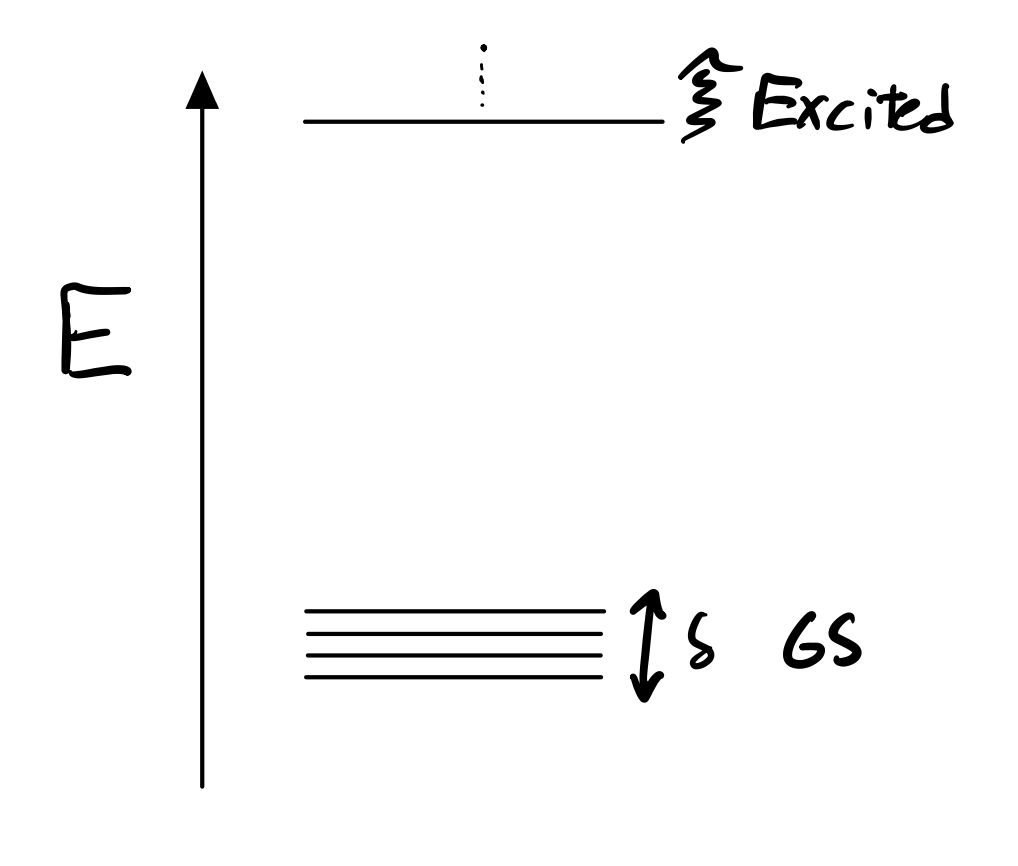
\includegraphics[scale=0.3]{Lectures/Images/lec3-gsmanifold.png}
\end{center}

\subsection{Argument for robustness}
Using the fact that $\set{W_1^X, W_2^X, W_1^Z, W_2^Z}$ (string operators) are flexible and non-commuting, we can establish a key property of the unperturbed ground states $\ket{\Omega, \pm}$. Namely, for any operator $O$ supported on less than $L$ sites:
\begin{equation}\label{eq:star}
    \bra{\Omega, \pm, \pm}O\ket{\Omega, \pm, \pm} = \text{diag}(c, c, c, c)
\end{equation}
for some constant $c$. A shorthand for the above is:
\begin{equation}
    \bra{\Omega, \alpha}O\ket{\Omega, \beta} = c\delta_{\alpha\beta}.
\end{equation}
You will show this relation on the homework.

Let's unpack this equation. The first thing it tells us is that:
\begin{equation}
    \bra{\Omega, \alpha}O\ket{\Omega, \alpha} = \bra{\Omega, \alpha'}O\ket{\Omega, \alpha'}
\end{equation}
which tells us that local operators cannot distinguish different ground states. The second thing it tells us is that:
\begin{equation}
    \bra{\Omega, \alpha'}O\ket{\Omega, \alpha} = 0 \quad \text{for }\alpha \neq \alpha'
\end{equation}
in other words, local operators cannot connect ground states.

As a comparison, consider $\ket{\uparrow}^{\otimes N}, \ket{\downarrow}^{\otimes N}$ the 2-fold degenerate ground states of the Ising model $H = -\sum_{ij}Z_iZ_j$. A local operator cannot connect them, but it is possible to distinguish the two states by measuring $Z_i$. In a symmetry breaking state, we do not have the structure of flexible strings, and hence do not have the same notion of local indistinguishability to arbitrary operators (only to symmetric ones).

Using the local distinguishability/unconnectability, let us sketch an argument for the toric code GSD. For concreteness, consider a perturbation:
\begin{equation}
    H' = H + \lambda \sum_j X_j.
\end{equation}
To obtain the first-order splitting (in degenerate perturbation theory), we need to find the matrix elements:
\begin{equation}
    \bra{\Omega, \pm, \pm}\sum_j X_j\ket{\Omega, \pm, \pm}
\end{equation}
and then diagonalize. By Eq. \eqref{eq:star}, we know that:
\begin{equation}
    \bra{\Omega, \pm, \pm}X_j\ket{\Omega, \pm, \pm} = c_j\II
\end{equation}
Therefore the ground state degeneracy is not split to first order. Looking at second order, we need to find matrix elements:
\begin{equation}
    \bra{\Omega, \pm, \pm}(\sum_j X_j)(H-E_{\text{gs}})^{-1}\Pi_{\text{ex}}(\sum_j X_j)\ket{\Omega, \pm, \pm}
\end{equation}
and then diagonalize (third, fourth order (and so on) we have the same procedure, just add a factor of $(H-E_{\text{gs}})^{-1}\Pi_{\text{ex}}(\sum_j X_j)$ each order). A given $X_j$ takes us to an excited state, the $\Pi_{\text{ex}}$ projector is then irrelevant\footnote{For a general operator, we instead can use that the projector can be restricted to a local operator as we only need to look at some local patch to tell that we are in an excited state}, and then $(H-E_{\text{gs}})^{-1}$ is just a number (difference between the ground and excited state energy), so we end up evaluating matrix elements of the form:
\begin{equation}
    \bra{\Omega, \pm, \pm}X_j X_k\ket{\Omega, \pm, \pm} = c\II
\end{equation}
where we again use Eq. \eqref{eq:star}. So, again at second order we have no splitting, and the argument follows the same way for third, fourth order etc. using the same property. The argument only breaks when the property no longer holds, which occurs at $L$th order of perturbation theory when we end up looking at the matrix element of an operator supported on $L$ sites. In particular, we get terms of the form:
\begin{equation}
    \prod_{j\in\hat{\gamma}_1}X_j = W_1^X, \quad \prod_{j\in\hat{\gamma}_2}X_j = W_2^X
\end{equation}
i.e. the string operators.

\begin{center}
    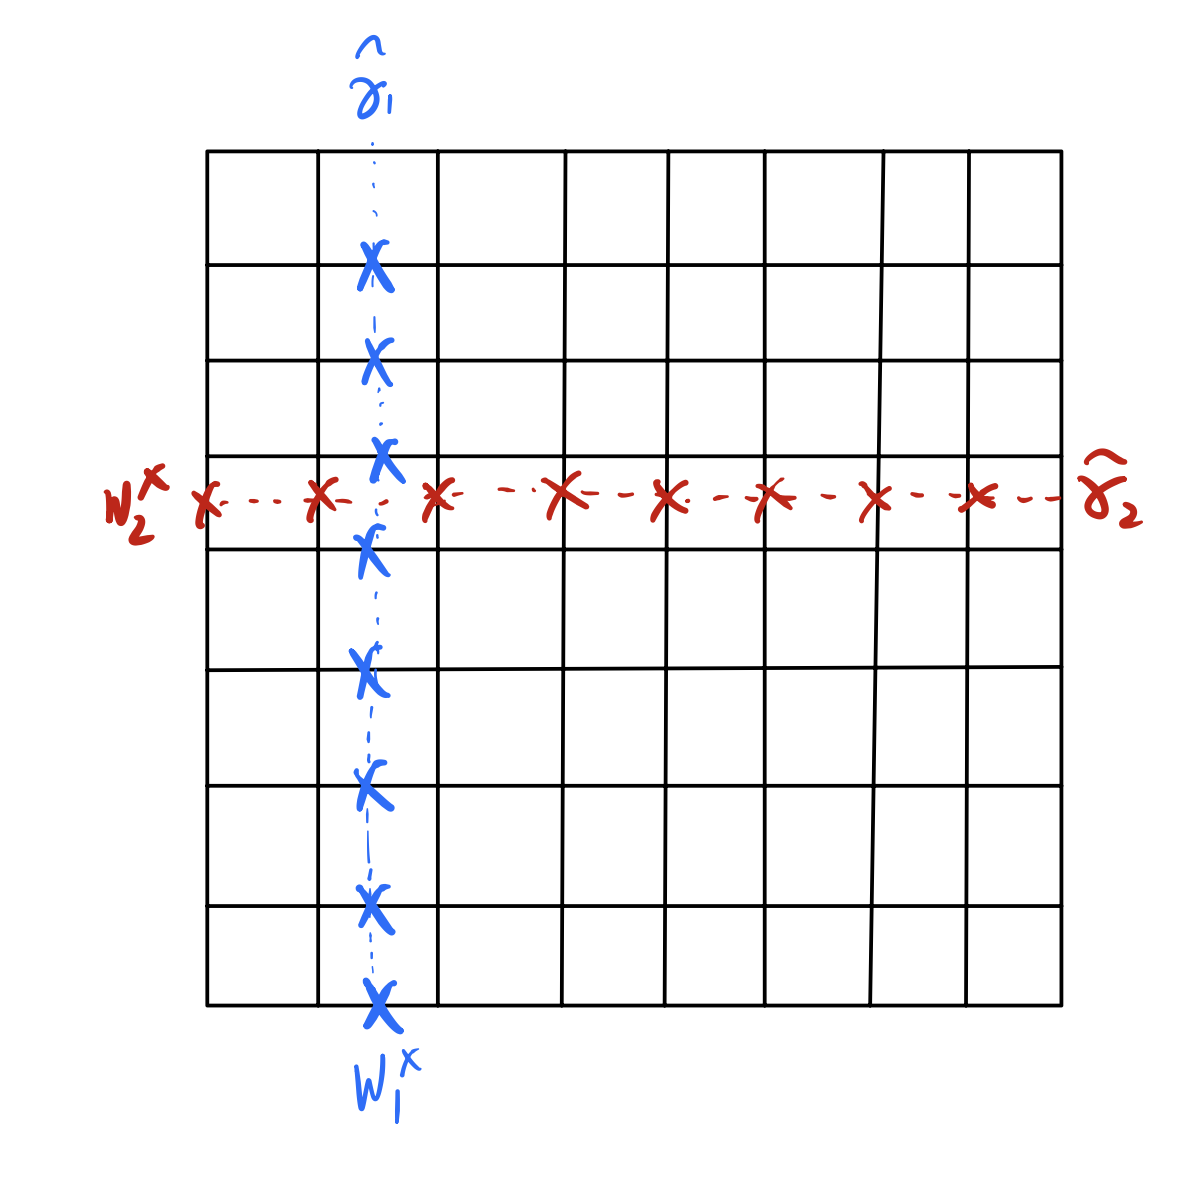
\includegraphics[scale=0.3]{Lectures/Images/lec3-strings.png}
\end{center}

Thus we end up the matrix elements:
\begin{equation}
    \bra{\Omega, \pm, \pm}W\ket{\Omega, \pm, \pm} \sim \lambda^L\text{diag}(c_1, c_2, c_3, c_4)
\end{equation}
and so then the splitting between the ground states is:
\begin{equation}
    \delta \sim \lambda^L = e^{-L\log(\frac{1}{\lambda})}
\end{equation}
Note that this is quite heuristic, and to make it rigorous you require more precise arguments, namely that the perturbation theory converges, with a finite radius of convergence $\lambda_0$ (which holds for arbitrarily large $L$). Without a formal argument, we expect such a finite radius of convergence for ``typical'' gapped local Hamiltonians, with $\lambda_0 \sim \Delta$ (so actually, in addition to the local indistinguishability, we are also using that the toric code is gapped).

\subsection{A Review of Berry Phase}
Before we move to a general discussion of anyons, we first review the notion of a Berry phase, which is a very related idea.

Let:
\begin{equation}
    \set{\ket{\psi(s)}, 0 \leq s \leq T, \ket{\psi(T)} = e^{i\phi}\ket{\psi(0)}}
\end{equation}
be a closed path in the set of normalized quantum states (rays in Hilbert space). Let us split up the path into $N$ parts of length $\Delta s$, with $N\Delta s = T$. Graphically:

\begin{center}
    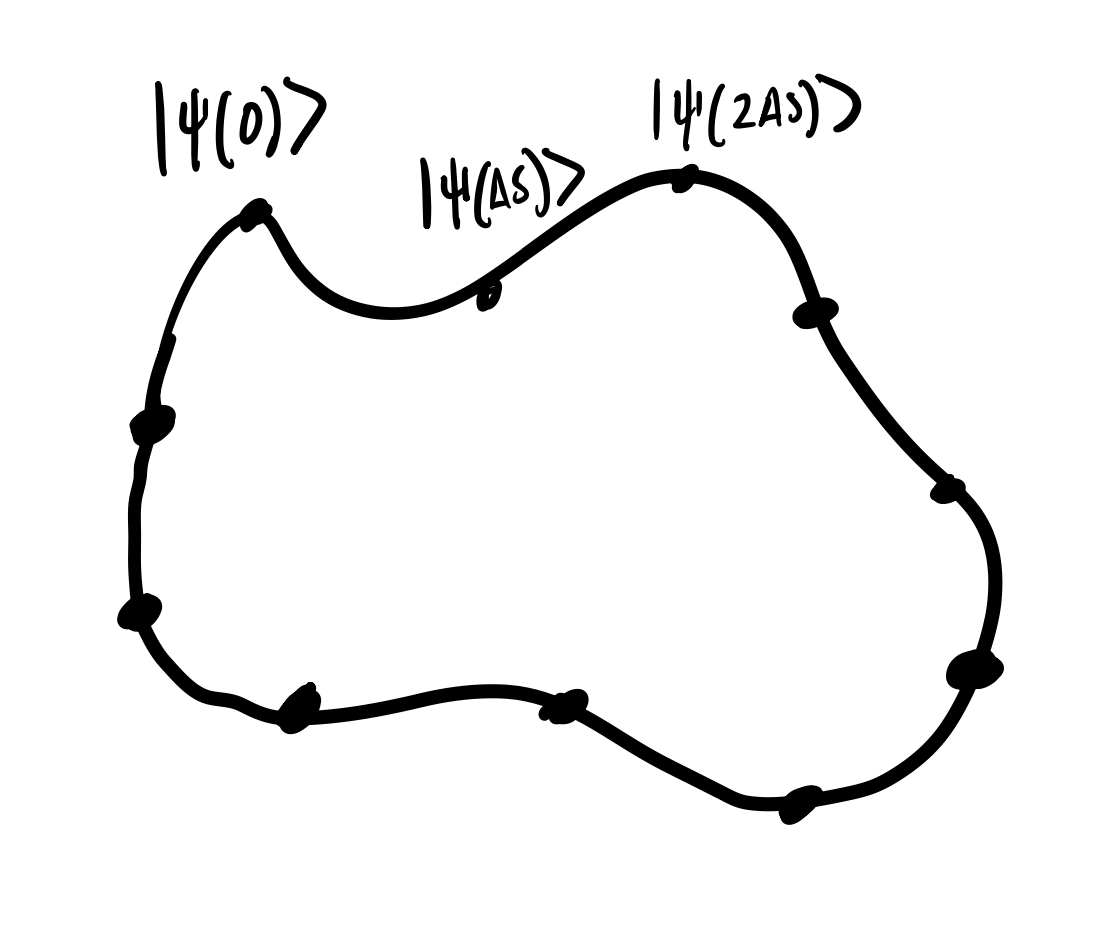
\includegraphics[scale=0.3]{Lectures/Images/lec3-berryphasepath.png}
\end{center}

and for brevity we denote $\ket{\psi(\cdot)} = \ket{\psi_\cdot}$. Now, we define the Berry phase as:
\begin{equation}
    e^{i\theta_B} = \lim_{N \to \infty}\braket{\psi_0}{\psi_{N-1}}\ldots\braket{\psi_2}{\psi_1}\braket{\psi_1}{\psi_0}
\end{equation}
The Berry phase has properties:
\begin{enumerate}
    \item $\abs{e^{i\theta_B}} = 1$, i.e. $e^{i\theta_B}$ is a $U(1)$ phase. This can be seen from the fact that $\braket{\psi_1}{\psi_0} \sim \frac{1}{N}$ and so the $N$-fold product is of order $\sim 1$.
    \item $e^{i\theta_B}$ only depends on the path and not its parameterization. That is, it is invariant under $s \to s' = f(s)$ with $f(0) = 0$ and $f(T) = T'$.
    \item $e^{i\theta_B}$ does not depend on the phase of $\ket{\psi(s)}$. That is, it is invariant under $\ket{\psi(s)} \to e^{i\varphi(s)}\ket{\psi(s)}$. This is easily seen from the definition - the phase of the ket is cancelled out by that of the bra in the $N$-fold product.
\end{enumerate}
Taking the limit $N \to \infty$, we have the formula:
\begin{equation}
    \theta_B = \int_0^T ds\phantom{i} i\bra{\psi(s)}\dod{}{s}\ket{\psi(s)}
\end{equation}
there is however the caveat when we evaluate the Berry phase in this way. We have to add the assumption that $\ket{\psi(0)} = \ket{\psi(T)}$ without the phase factor.

\subsection{Berry phase and adiabatic evolution}
The Berry phase shows up in two places; in adiabatic processes/cycles, and in path integrals. Today, we talk about the former.

First, a reminder of the adiabatic theorem. Let $H(t)$ be a time-dependent Hamiltonian with $0 \leq t \leq T$. Suppose $H(t)$ has a unique ground state $\ket{\psi(t)}$ with energy $E(t)$ and gap $\Delta(t)$. Suppose $H(t)$ varies on a timescale $\tau \gg \frac{1}{\min_t \Delta (t)}$. Then:
\begin{equation}
    \ket{\psi(0)} \stackrel{\text{evolve under } H(t)}{\longrightarrow} (\text{phase})\ket{\psi(t)}.
\end{equation}

Now, consider a closed path $H(T) = H(0)$, which we may consider an ``adiabatic cycle''. 

\begin{center}
    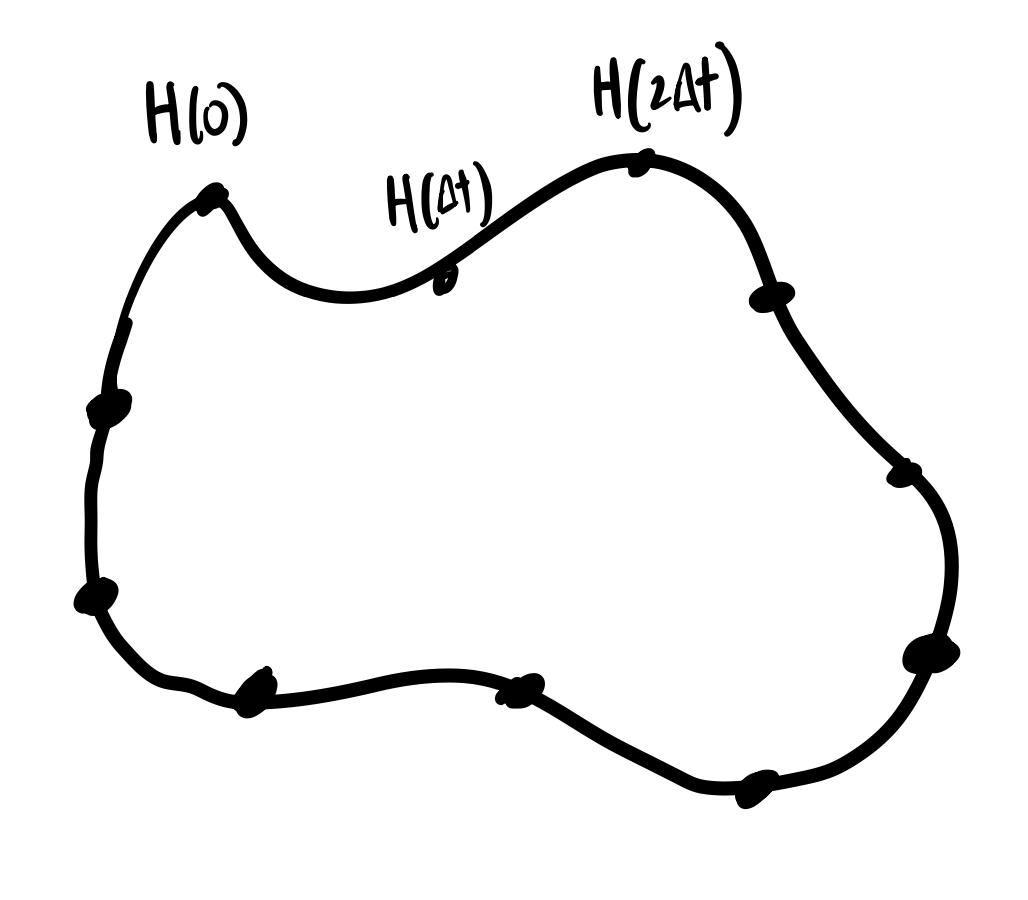
\includegraphics[scale=0.3]{Lectures/Images/lec3-Hpath.png}
\end{center}

Then:
\begin{equation}
    \ket{\psi(0)} \stackrel{\text{evolve}}{\longrightarrow} (\text{phase})\ket{\psi(0)}
\end{equation}
Let's compute this phase factor! It is given by:
\begin{equation}
    (\text{phase}) = \bra{\psi(0)}\mathcal{T}\exp(-i\int_0^T dt H(t))\ket{\psi(0)}
\end{equation}
with $\mathcal{T}$ denoting time ordering. We compute the phase factor by discritizing the time-dependent Hamiltonian to $H(0) = H_0, H(\Delta t) = H_1, H(2\Delta t) = H_2, \ldots$ with $N\Delta t = T$ and associated instantaneous ground states $\ket{\psi(0)} = \ket{\psi_0}, \ket{\psi(\Delta t)} = \psi_1, \ldots$. Then the expression for the phase factor becomes:
\begin{equation}
    (\text{phase}) = \lim_{N \to \infty }\bra{\psi(0)}e^{-i\Delta tH_{N-1}}e^{-i\Delta tH_{N-2}}\ldots e^{-i\Delta tH_{1}}e^{-i\Delta tH_{0}}\ket{\psi(0)}
\end{equation}
According to the adiabatic theorem, we know that:
\begin{equation}
    e^{-i\Delta t H_0}\ket{\psi_0} = \dyad{\psi_1}{\psi_1}e^{-i\Delta t H_0}\ket{\psi_0}
\end{equation}
as the adiabatic evolution takes $\ket{\psi_0} \to \ket{\psi_1}$ in the first time interval. We can thus insert projectors about each time step:
\begin{equation}
    (\text{phase}) = \lim_{N \to \infty }\bra{\psi(0)}e^{-i\Delta tH_{N-1}}\dyad{\psi_{N-1}}{\psi_{N-1}}e^{-i\Delta tH_{N-2}}\dyad{\psi_{N-2}}{\psi_{N-2}}\ldots \dyad{\psi_{2}}{\psi_{2}}e^{-i\Delta tH_{1}}\dyad{\psi_{1}}{\psi_{1}}e^{-i\Delta tH_{0}}\ket{\psi(0)}
\end{equation}
Each of the expectation values only gives a phase factor of the energy, and so:
\begin{equation}
    (\text{phase}) =  \lim_{N \to \infty }\exp(-i\Delta t \sum_{k=0}^{N-1}E_k)\braket{\psi_0}{\psi_{N-1}}\ldots\braket{\psi_2}{\psi_1}\braket{\psi_1}{\psi_0}
\end{equation}
and so:
\begin{equation}
    \boxed{(\text{phase}) = \exp(-i\int_0^T E(t)dt)e^{i\theta_B}}
\end{equation}
i.e. we have a path-dependent dynamical phase part and a Berry phase part.

We'll stop here for now, and next time we will discuss the Berry phase associated with anyons.